\documentclass[a4paper,10pt,notitlepage]{article}
\usepackage{sprawozdanie-ato}


\begin{document}


\title{\
Laboratorium Sieci Komputerowych\\\
Protokoły \arp{} i \ppp{}
}
\author{\
Tomasz Cudziło, Barnaba Turek\\
\textsc{PW EE Informatyka}\\[6pt]
}
\date{\today}

\maketitle
\tableofcontents


\section{Cel ćwiczenia}

W ramach laboratorium mieliśmy za zadanie zbadać działanie protokołu \arp,
oraz skonfigurować połączenie pomiędzy dwoma maszynami korzystając z protokołu
\ppp.


\section{Wykonanie ćwiczenia}

\subsection{Wstęp}

\arp{} -- \emph{Address Resolution Protocol} jest protokołem umożliwiającym
współpracę pomiędzy drugą a trzecią warstwą modelu OSI. Jest wykorzystywany do
znajdywania adresów maszyn w warstwie łącza, na podstawie ich adresów w warstwie
sieci. W wykonanym ćwiczeniu znajdowany zostaje adres MAC maszyny, posiadając
jej adres IPv4.

Zasada działania protokołu \arp{} jest stosunkowo prosta. W systemach
operacyjnych protokół obsługiwany jest przeważnie przez program \texttt{arp}.
Gdy adres fizyczny maszyny\dywiz adresata jest nieznany, wysyłane jest zapytanie
\arp. Jest to ramka \eth{} zawierająca adres IP adresata. Ramka jest prośbą o
odpowiedź od maszyny, która ma przypisany dany adres IP
\cite{arp:stevens_arp_przyklad}. Zapytanie jest wysyłanie jako \emph{broadcast}
na warstwie łącza aktualnej podsieci.

Dla polepszenia wydajności zarządzania połączeniami, program \texttt{arp}
przechowuje w pamięci podręcznej tablicę mapującą adresy logicznie na adresy
fizyczne. Wpis jest uznawany za poprawny przez okres 20 minut, następnie zostaje
odświeżony \cite{arp:stevens_arp_cache}.

W sieciach IPv6 funkcjonalność \arp{} spełnia protokół NDP -- \emph{Neighbor
Discovery Protocol}. W połączeniach \ppp{} i innych połączeniach point-to-point
protokół \arp{} nie jest potrzebny.

\subsection{Wykonanie ćwiczenia}

Korzystano z maszyn \tjz{} (\texttt{t10}) oraz \tjj{} (\texttt{t11}) połączonych
bezpośrednio kablem \eth. Schemat nr.~\ref{fig:arp:schemat-po-konfiguracji}
przedstawia wykorzystane połączenia.

\begin{figure}[h!]
  \centering
  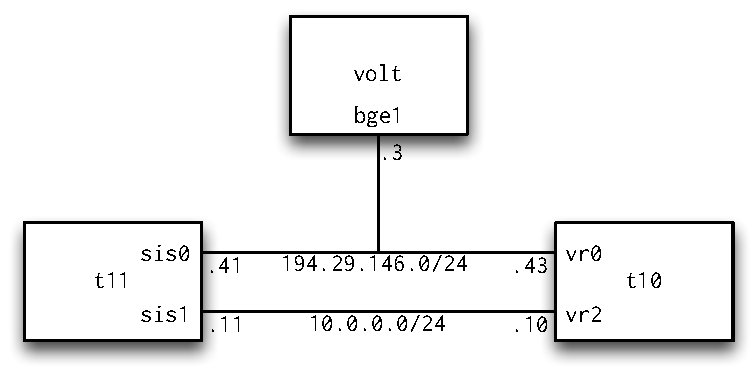
\includegraphics[width=11cm]{figury/arp/schemat-po-konfiguracji.pdf}
  \caption{Schemat sieci IPv4 do obserwacji \arp.}
  \label{fig:arp:schemat-po-konfiguracji}
\end{figure}

Interfejsy maszyn należące do sieci \texttt{194.29.146.0/24} tj. \texttt{sis0}
oraz \texttt{vr0} odpowiednio dla maszyn \tjz{} oraz \tjj, zostały
prekonfigurowane podczas podnoszenia systemu operacyjnego. Sieć
\texttt{10.0.0.0/24} została skonfigurowana do obserwacji pakietów protokołu
\arp. Na obu maszynach ręcznie skonfigurowano interfejsy, oraz upewniono się, że
pamięć podręczna \texttt{arp} jest pusta.

\begin{lstlisting}
so5501b% sudo ifconfig vr2 10.0.0.10/24
so5501b% sudo arp -d -i vr2 -a
so5501b% arp -i vr2 -a
? (10.0.0.10) at SO5501B2 on vr2 permanent [ethernet]
\end{lstlisting}

\begin{lstlisting}
so4801% sudo ifconfig sis1 10.0.0.11/24
so4801% sudo arp -d -i sis1 -a
so4801% arp -i sis1 -a
? (10.0.0.11) at SO4801B on sis1 permanent [ethernet]
\end{lstlisting}

Włączono nasłuchiwanie pakietów \arp{} na \tjj{} i przesłano jedno zapytanie
\texttt{ping} z maszyny \tjz.

\begin{lstlisting}
so5501% ping -c 1 10.0.0.11
\end{lstlisting}

\begin{lstlisting}
so4801% sudo tcpdump -i sis1 arp
listening on sis1, link-type EN10MB (Ethernet), capture size 65535 bytes
17:08:50.072670 ARP, Request who-has 10.0.0.10 tell 10.0.0.11, length 28
17:08:50.072865 ARP, Reply 10.0.0.10 is-at SO5501B2, length 46
17:13:16.147967 ARP, Request who-has 10.0.0.11 tell 10.0.0.10, length 46
17:13:16.148178 ARP, Reply 10.0.0.11 is-at SO4801B, length 28
\end{lstlisting}

W listingu widoczne są dwie wymiany \texttt{Request/Reply}. Pierwsza z maszyny
\tjz{} szukającej maszyny \tjj{}, by wysłać zapytanie z \texttt{ping}. Druga
wymiana, jest z maszyny \tjj{}, by móc odpowiedzieć na \texttt{ping}.

\subsection{\ppp}


\subsubsection{Wstęp}

\ppp{} -- \emph{Point-to-Point Protocol} to rozwiązanie służące do
przenoszenia datagramów IP. Najczęściej jest stosowany do tworzenia połączeń
opartych na połączeniach szeregowych takich jak modemy, łącza
optyczne\cite{ppp:stevens-ppp}.

W przeciwieństwie do \arp{} \ppp{} należy traktować raczej jako zbiór
protokołów. Protokoły te pozwalają między innymi na utworzenie połączenia
\ppp{} (LCP), oraz konfigurację połączenia, które będzie korzystać z
połączenia \ppp{} (NCP) --- na przykład połączenia \ip.

Zakresem działania LCP -- \emph{Link Control Protocols} jest samo zestawienie
połączenia pomiędzy dwoma urządzeniami. Wymagania wobec połączenia są
minimalne w stosunku do innych protokołów, wystarczy wsparcie dla komunikacji
dwukierunkowiej.

\ppp{} nie koncentruje się na zapewnieniu niezawodności połączenia i
retransmisji danych. Istnieją standardy i protokoły, które mogą rozwiązywać
problemy z niezawodnością sieci w ramach \ppp{}. To zadanie jest delegowane do
protokółu, który działa wewnątrz połączenia \ppp{}, np. \ip{}. Istnieją też
protokoły i rozszerzenia \ppp{} wspierające szyfrowanie, kompresję i
raportowanie stanu połączenia.

Ponieważ stacja robocza na laboratorium nie była wyposażona w modem, w ramach
ćwiczenia \ppp{} wykonaliśmy połączenie \tcp{} poprzez \pppoe{}. Zwykle
połączenia tego typu stosowane są do połączenia z modemem lub podobnym
urządzeniem poprzez sieć LAN lub WAN \cite{ppp:stevens-pppoe}. Ostatecznie na
łączu ethernetowym można zestawić połączenie \tcp{} nie korzystając z \ppp{}.


\subsubsection{Przygotowanie ćwiczenia}

Konfiguracja sprzętowa połączenia przedstawiała się następująco:

\begin{figure}[h!]
  \centering
  
\includegraphics[width=11cm]{figury/ppp/schemat-przed.pdf}
  \caption{Schemat sieci dla połączenia \ppp.}
  \label{fig:ppp:schemat-sieci-przed}
\end{figure}

Maszyny \pppcli{} i \pppserv{} połączyliśmy skrosowanym kablem.

Zaczęto od rekonfiguracji interfejsów \texttt{sis2} i \texttt{fxp0} do potrzeb
ćwiczenia. Następnie podniesiono te interfejsy.

Maszyna \pppserv{} pełniła rolę serwera \ppp, a maszyna \pppcli{} rolę klienta
\ppp. Na maszynie \pppcli{} skonfigurowano połączenie w taki sposób, aby
wynegocjowane zostało następujące połączenie \tcp{}:

\begin{figure}[h!]
  \centering
  
\includegraphics[width=11cm]{figury/ppp/schemat-po.pdf}
  \caption{Schemat sieci tunelowanej przez \ppp.}
  \label{fig:ppp:schemat-sieci-po}
\end{figure}


\subsubsection{Wykonanie ćwiczenia}

Skonfigurowano klienta \ppp{} na maszynie \pppcli{} w następujący sposób:

\begin{lstlisting}
#/etc/ppp/ppp.conf
default:
  # Logowanie
  set log Phase tun command

polaczenie:
  # Docelowa konfiguracja sieci
  set ifaddr 10.0.0.1/0 10.0.0.2/0

  # Urzadzenie, z ktorego PPP ma korzystac
  # Suffix ':*' oznacza, ze klient powinien probowac nawiazac polaczenie
  # z dowolnym providerem
  set device PPPoE:fxp0:* #1

  set authname ppp
  set authkey ppp
  set dial
  set login
  add default HISADDR
\end{lstlisting}

Następnie na \pppserv{} uruchomiono proces \texttt{pppoed}:

\begin{lstlisting}
t10$ sudo service pppoed onestart sis2
\end{lstlisting}

Na \pppcli{} wykonano komendę zestawiającą połączenie. Wynik polecenia
\texttt{ifconfig} następnie pokazuje nowe połączenie.

\begin{lstlisting}
k11$ ppp -ddial polaczenie
k11$ ifconfig tun0
tun0: flags=8051<UP,POINTOPOINT,RUNNING,MULTICAST> metric 0 mtu 1492
        options=80000<LINKSTATE>
        inet 10.0.0.2 --> 10.0.0.1 netmask 255.255.255.255
        Opened by PID 27226
\end{lstlisting}


\subsubsection{Obserwacja połączenia i wnioski}

Udało się zaobserwować negocjację połączenia przez protokół LCP. Maszyna
\pppserv{} nazywała się wtedy \texttt{so5501b}.

\begin{lstlisting}
17:36:01.655628 PPPoE PADI [Host-Uniq 0xC0B9C5C2] [Service-Name "*"]
17:36:34.096172 PPPoE PADI [Host-Uniq 0x803AD9C2] [Service-Name "*"]
17:36:34.102227 PPPoE PADO [AC-Name "so5501b"] [Service-Name "*"]
    [Host-Uniq 0x803AD9C2] [AC-Cookie 0x400818C3]
17:36:34.102367 PPPoE PADR [Host-Uniq 0x803AD9C2]
    [AC-Cookie 0x400818C3] [AC-Name "so5501b"] [Service-Name "*"]
17:36:34.102455 PPPoE PADS [ses 0x1] [AC-Name "so5501b"]
    [Service-Name "*"] [Host-Uniq 0x803AD9C2] [AC-Cookie 0x400818C3]
17:36:35.365394 PPPoE [ses 0x1] LCP, Conf-Request (0x01), id 1, length 26
17:36:35.365863 PPPoE [ses 0x1] LCP, Conf-Request (0x01), id 1, length 26
17:36:35.365913 PPPoE [ses 0x1] LCP, Conf-Ack (0x02), id 1, length 26
17:36:35.366971 PPPoE [ses 0x1] LCP, Conf-Ack (0x02), id 1, length 26
\end{lstlisting}

Jest to zgodne ze schematem negocjacji opisanej w \cite{ppp:stevens-pppoe}:

\begin{figure}[h!]
  \centering
  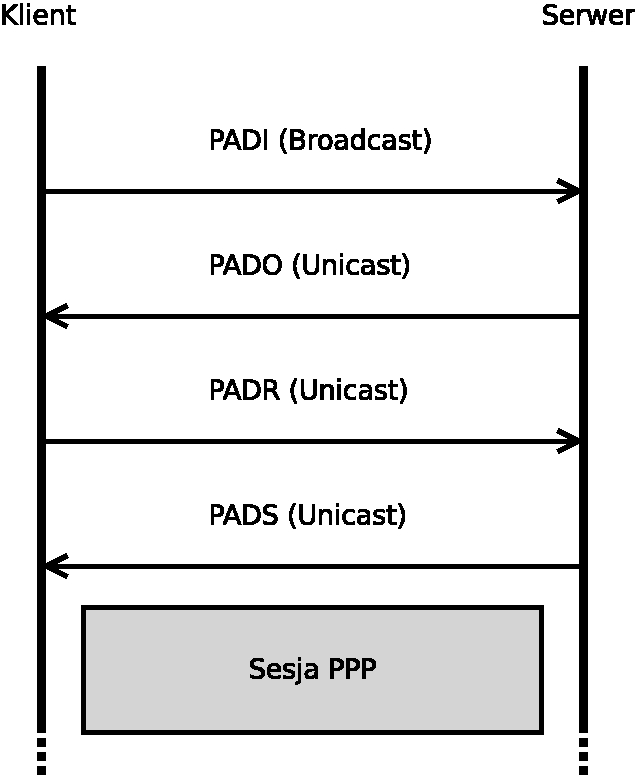
\includegraphics[width=5cm]{figury/ppp/padi-pado.pdf}
  \caption{Negocjacja połączenia \ppp.}
  \label{fig:ppp:schemat-sieci-przed}
\end{figure}

Po ustanowieniu sesji można zauważyć, że protokół LCP zaczyna konfigurować
połączenie \tcp{} zgodnie z konfiguracją w pliku \texttt{/etc/ppp/ppp.conf}.
Za pomocą poleceń \texttt{ping} i \texttt{netcat} potwierdzono, że połączenie
faktycznie działa.

\begin{lstlisting}
17:40:27.658383 PPPoE [ses 0x3] IP so4801c.iem.pw.edu.pl > 10.0.0.1: ICMP echo request, id 61802, seq 0, length 64
17:40:27.660076 PPPoE [ses 0x3] IP 10.0.0.1 > so4801c.iem.pw.edu.pl: ICMP echo reply, id 61802, seq 0, length 64
17:40:28.657813 PPPoE [ses 0x3] compressed PPP data
17:40:28.658171 PPPoE [ses 0x3] compressed PPP data
\end{lstlisting}

Widoczne jest zestawione połączenie z kompresją --- przynajmniej według
programu \texttt{tcpdump}. Można też zaobserwować pakiety zarówno przed, jak i
po opakowaniu w ramki \ppp{}. Program \texttt{tcpdump} nie pozwala jednak
zobaczyć, co dokładnie jest w pakietach przenoszonych przez \ppp.



%\section{Bibliografia}

\begin{thebibliography}{99}
    \bibitem{arp:stevens_arp_przyklad}
        \emph{TCP/IP Illustrated --- 2nd ed.}; Kevin R. Fall, W. Richard Stevens; Pearson Education, Inc.
        Rozdział 4.2
    \bibitem{arp:stevens_arp_cache}
        \emph{TCP/IP Illustrated --- 2nd ed.}; Kevin R. Fall, W. Richard Stevens; Pearson Education, Inc.
        Rozdział 4.3
\end{thebibliography}



\end{document}
